\documentclass[a4paper, 12pt]{article}

\newcommand{\templates}{../../template}
\usepackage[a4paper, margin=2.5cm]{geometry}

\usepackage{enumitem}
\setlist[itemize]{noitemsep}
\setlist[enumerate]{noitemsep}

\let\oldpar\paragraph
\renewcommand{\paragraph}[1]{\oldpar{#1\\}\noindent}
\usepackage{graphicx}
\usepackage{hyperref}
\usepackage{makecell}

\newcommand{\settitolo}[1]{\newcommand{\titolo}{#1\\}}
\newcommand{\setprogetto}[1]{\newcommand{\progetto}{#1\\}}
\newcommand{\setcommittenti}[1]{\newcommand{\committenti}{#1\\}}
\newcommand{\setredattori}[1]{\newcommand{\redattori}{#1\\}}
\newcommand{\setrevisori}[1]{\newcommand{\revisori}{#1\\}}
\newcommand{\setresponsabili}[1]{\newcommand{\responsabili}{#1\\}}
\newcommand{\setversione}[1]{
	\ifdefined\versione\renewcommand{\versione}{#1\\}
	\else\newcommand{\versione}{#1\\}\fi
}
\newcommand{\setdestuso}[1]{\newcommand{\uso}{#1\\}}
\newcommand{\setdescrizione}[1]{\newcommand{\descrizione}{#1\\}}

\newcommand{\makefrontpage}{
	\begin{titlepage}
		\begin{center}

		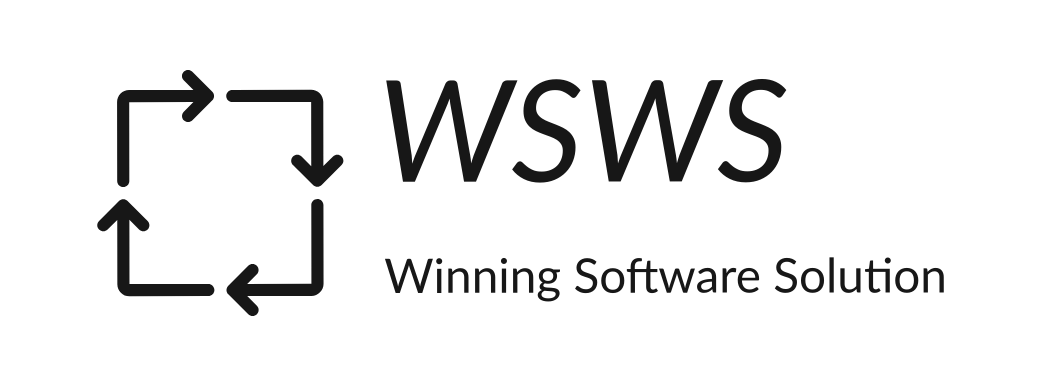
\includegraphics[width=0.4\textwidth]{../../template/WSWS-logos_transparent_crop}\\

		{\Large Winning Software Solution}\\[6pt]
		\href{mailto://winningsoftwaresolution@gmail.com}{winningsoftwaresolution@gmail.com}\\
		
		\ifdefined\progetto
		\vspace{1cm}
		{\Large\progetto}
		{\large\committenti}
		\else\fi
		
		\vspace{1.5cm}
		{\LARGE\titolo}
		
		\vfill
		
		\begin{tabular}{r | l}
		\multicolumn{2}{c}{\textit{Informazioni}}\\
		\hline
		
		\ifdefined\redattori
			\textit{Redattori} &
			\makecell[l]{\redattori}\\
		\else\fi
		\ifdefined\revisori
			\textit{Revisori} &
			\makecell[l]{\revisori}\\
		\else\fi
		\ifdefined\responsabili
			\textit{Respondabili} &
			\makecell[l]{\responsabili}\\
		\else\fi
		
		\ifdefined\versione
			\textit{Versione} & \versione
		\else\fi
		
		\textit{Uso} & \uso
		
		\end{tabular}
		
		\vspace{2cm}
		
		\ifdefined\descrizione
		Descrizione
		\vspace{6pt}
		\hrule
		\descrizione
		\else\fi
		\end{center}
	\end{titlepage}
}
\usepackage{hyperref}
\usepackage{array}
\usepackage{tabularx}

\def\vers#1-#2-#3-#4-#5\\{#1&#2&#3&#4&#5\\\hline}

\newcommand{\addversione}[5]{
	\ifdefined\versioni
		\let\old\versioni
		\renewcommand{\versioni}{#1&#2&#3&#4&#5\\\hline\old}
	\else
		\newcommand{\versioni}{#1&#2&#3&#4&#5\\\hline}
	\fi
}

\newcommand{\setversioni}[1]{\newcommand{\versioni}{#1}}

\newcommand{\makeversioni}{
	\begin{center}
		\begin{tabularx}{\textwidth}{|c|c|c|c|X|}
		\hline
		\textbf{Versione} & \textbf{Data} & \textbf{Persona} & \textbf{Attivtà} & \textbf{Descrizione} \\
		\hline
		\versioni
		\end{tabularx}
	\end{center}
	\clearpage
}

%package
\usepackage[table,xcdraw]{xcolor}

\settitolo{Analisi delle tecnologie}
\setredattori{Federico Marchi \\ Matteo Galvagni}
\setdestuso{Esterno}
\setdescrizione{
Analisi delle tecnologie.
}

\begin{document}

\makefrontpage

\section{Analisi delle Blockchain}

\subsection*{Premesse}
Le metriche di valutazione sono state scelte in base alla loro importanza sia nella normale valutazione di una blockchain sia nello svolgimento di questo particolare progetto.
È importante tenere in considerazione che, mentre alcune delle metriche sono dati di fatto, altre sono stime empiriche o valori dichiarati dagli sviluppatori ma mai dimostrati.
Di seguito una rapida spiegazione di ogni metrica scelta.

\subsubsection*{Scalabilità}
Gli attributi scelti per valutare la scalabilità di ogni blockchain mirano non solo a dare un'idea della velocità e dei costi attuali per operare su ogni rete, ma anche a stimare come tale
rete potrebbe performare in futuro e/o in periodi di congestione per via di un ipotetico aumento della domanda di utilizzo.

\begin{itemize}
\item \textbf{Transaction fee: }
È il costo medio \textit{attuale} per effettuare una normale transazione sulla rete.
È un costo personalizzabile: nulla vieta infatti di impostare un costo più alto del normale per assicurarsi una velocità di transazione maggiore o viceversa.
Questa metrica è fondamentale per una buona riuscita del progetto in esame, in quanto è assolutamente preferibile che al momento della scannerizzazione del codice QR
il cliente paghi una cifra insignificante (idealmente, nell'ordine dei centesimi o inferiore) per chiamare la funzione dello \textit{smart contract} che si occuperà di sbloccare i fondi
al venditore. È inoltre preferibile, ma meno significativo del precedente esempio, che anche in fase d'acquisto la tassa di transazione sia molto bassa, anche se
in questa particolare fase una tassa di poche decine di centesimi è considerata accettabile in quanto pressoché in linea con il costo della competizione (Es.: prezzo di un bonifico;
tassa percentuale trattenuta da servizi come \textit{Paypal}).
È inoltre necessario esaminare come il costo per transazione cambierebbe in caso di un aumento della domanda di utilizzo della blockchain, per garantire un funzionamento
accettabile anche nel futuro.\\

\item \textbf{Transaction time: }
Anche detta \textit{Transaction finality}, è il tempo medio \textit{attuale} in cui una transazione viene confermata e inserita permanentemente nella blockchain.
Esso è la somma del tempo in cui la transazione, una volta emessa, viene accettata da un miner/validatore inserendola in un blocco e il tempo impiegato da tale blocco per essere
approvato (block time). Dipende direttamente dalla tassa di transazione: se viene impostato un costo molto più alto del normale i miners/validatori saranno incentivati a includere tale transazione
in un blocco e approvare quel blocco il prima possibile, così da aggiudicarsi la tassa di transazione. Al contrario, una tassa impostata per risultare in una transazione più economica
sarà scelta per ultima dai miners/validatori, in quanto non hanno incentivo economico ad approvare tale transazione prima di altre che pagano di più.
Per il progetto in esame è fondamentale un tempo di transazione molto basso (idealmente nell'ordine dei secondi) poichè il cliente nella fase di scannerizzazione del codice QR deve
avere un'esperienza veloce.\\

\newpage

\item \textbf{Block time: }
È il tempo medio \textit{attuale} in cui un blocco viene approvato nella blockchain. Indica la velocità con quale i miners/validatori di una rete approvano un blocco e va valutato insieme al parametro "grandezza di blocco": un blocco molto grande può contenere molte transazioni, quindi anche con un tempo di blocco non esemplare il tempo di transazione diminuisce considerevolmente
perchè molte più transazioni possono essere incluse in un blocco, anche quelle che eventualmente rendono meno profitto ai miners/validatori; al contrario, un blocco molto piccolo (anche se con velocità
di approvazione eccellente) causa problemi altrove poichè molte meno transazioni possono essere incluse nel blocco creando forte competizione per ottenere l'approvazione della transazione risultando
in transazioni con costi impostati per essere medio-bassi molto più lente.\\

\item \textbf{Block size: }
È il peso in memoria di un blocco. È proporzionale al numero di transazioni che un blocco può contenere: un blocco molto grande risulta in TPS (\textit{Transactions per second}) elevate e un costo per transazione
moderato/basso poichè vi è poca competizione da parte delle transazioni per essere inserite nel blocco, come spiegato nel punto precedente. Un blocco molto grande, invece, richiederebbe una velocità di connessione e soprattutto una velocità di memorizzazione dei blocchi non indifferenti nei periodi di massimo utilizzo della rete al fine di emettere i blocchi e sincronizzare il nodo in tempo utile per ricevere il compenso economico, spingendo i nodi con requisiti hardware non sufficienti e quindi non economicamente incentivati a non fornire più il loro servizio risultando in una centralizzazione della blockchain.
È importante considerare che vi è un dibattito aperto riguardo la grandezza \textit{limite} di un blocco: blocchi estremamente piccoli risultano in costi di transazione molto alti in periodi di grande utilizzo della rete, ma sono facilmente minabili/validabili senza requisiti hardware eccessivi e non rappresentano quindi un potenziale pericolo per la decentralizzazione come invece fanno
dei blocchi molto grandi, che di contro garantiscono costi di transazione bassi e maggiori TPS. Riteniamo che entrambe le argomentazioni siano più che valide, dunque nella
valutazione finale verrà cercato un compromesso tra le due visioni del problema.\\

\item \textbf{TPS: }
È il numero \textit{massimo teorico} di transazioni che una rete può processare in un secondo.
È una metrica utile per valutare se una rete ha la capacità di elaborare una mole importante di transazioni che potrebbe dover affrontare in futuro senza
congestionarsi e dunque richiedere costi di transazione eccessivi.
Va sottolineato che è un valore puramente \textit{teorico} e non riflette per forza la reale capacità di carico di una rete.
Alcune di queste misurazioni, infatti, sono state fatte in ambiente di test (\textit{testnet}) dove la velocità di approvazione dei blocchi è
generalmente molto maggiore di quella della rete reale, in quanto l'ambiente di test è spesso estremamente centralizzato e offre hardware dedicato.

\end{itemize}

\newpage

\subsubsection*{Sicurezza \& Decentralizzazione}
Le metriche di valutazione della sicurezza e della decentralizzazione vogliono invece dare una stima teorica del livello di resistenza di ogni rete a possibili attacchi da parte di entità
malevole. I tipi di attacchi possono avere natura diversa: è necessario che la rete scelta sia protetta sia da attacchi di tipo economico (Es.: gli sviluppatori vendono una grande quantità
di token nativi nel tentativo di intascare il denaro degli investitori; un'entità include una transazione malevola (spesa
di token non posseduti) in un blocco e riesce a minarlo/validarlo) sia da attacchi mirati alla distruzione della rete (Es.: uno o pochi stati vietano il mining/la validazione dei blocchi
e la rete perde gran parte o la totalità dei suoi nodi; un'azienda che controlla gran parte dei miners/validatori chiude o viene a sua volta attaccata e l'intera rete va offline).

\begin{itemize}

\item \textbf{Consensus: }
Si tratta dell'algoritmo utilizzato dalla rete per raggiungere un consenso su quali blocchi siano effettivamente validi.
Principalmente esistono due meccanismi di consenso ritenuti validi: \textit{Proof of Work} e \textit{Proof of Stake}.

\begin{itemize}
    \item \textbf{Proof of Work: }
    In sintesi, un blocco viene approvato (minato) quando viene trovato un particolare numero che, se messo in coda alla lista delle transazioni, una funzione di hash che prende
    in input la lista seguita da quel numero restituisce un output atteso dal protocollo. Per esempio, analizzando il \textit{whitepaper} di Bitcoin, si scopre che
    l'output in binario che deve restituire la funzione di hash deve avere il numero arbitrario di 30 zeri in testa.
    Siccome la funzione di hash scelta è un problema in NP, mentre è computazionalmente facile accorgersi se l'output è corretto dato il numero in input, è invece estremamente difficile
    trovare il numero in input che genera l'output desiderato (assumendo che non esista un algoritmo più efficiente del bruteforce, il che non è dimostrato teoricamente ma è l'assunzione su cui si basa il mining). Il miner che fornisce il numero che genera l'output atteso dal protocollo
    avrà dunque impiegato molte risorse hardware per trovarlo.
    Una volta che un miner "dichiara" di aver trovato il numero corretto, tutti i nodi connessi effettuano un rapido test per stabilire se l'output è quello atteso, procedendo
    poi con un voto democratico per includere il blocco nella blockchain.
    Sapendo che validare i blocchi è computazionalmente difficile (sempre assumendo che non esista algoritmo migliore del bruteforce), si può garantire la sicurezza della rete da attacchi da parte di entità malevole: per controllare il 50\% + 1 della
    rete al fine di approvare blocchi fraudolenti è necessaria un'enorme potenza computazionale e dunque un'enorme disponibilità economica.\\

    \item \textbf{Proof of Stake: }
    In questo tipo di consenso, invece, validare i blocchi non è computazionalmente difficile. La sicurezza deriva dal fatto che per diventare validatore è necessario uno
    \textit{stake} di token nativi che sono bloccati e non spendibili durante l'attività da validatore. Mente esistono più variazioni di questo meccanismo che vanno approfondite, generalmente il funzionamento segue la seguente procedura.
    Ad ogni blocco viene scelto (anche detto "eletto") un numero arbitrario di validatori tra tutti i validatori "candidati" online, questo gruppo
    ha il compito di validare rapidamente le transazioni ed emettere un blocco corretto.
    Se viene emesso un blocco fraudolento o se un validatore eletto va offline, parte dei token bloccati di quel validatore sono distrutti e persi per sempre.
    \newpage
    Vi è quindi un forte incentivo economico a non emettere blocchi non validi e a rimanere online. Inoltre, per appropriarsi della rete è necessaria
    una disponibilità economica enorme per creare un numero significativo di validatori (considerando anche che non basta avere metà dei validatori candidati, è anche necessario che più della metà dei validatori eletti siano tra quelli), e anche se un'entità provasse un attacco del genere i soldi spesi per l'acquisto dei token sarebbero persi per sempre poichè se la rete collassasse il valore dei suoi token nativi collasserebbe con lei.\\

\end{itemize}

\item \textbf{Miners/Validators: }
È il numero di miners (nelle blockchain con PoW) o validatori (nelle blockchain PoS) attualmente online.
Una blockchain con pochi nodi è sicuramente più veloce, poichè meno nodi devono sincronizzare e votare per l'approvazione dei blocchi, ma è
anche poco decentralizzata e quindi poco protetta da attacchi mirati da parte di entità o addirittura governi.
Oltre ad essere un chiaro indicatore di quanto una rete è effettivamente decentralizzata, questa metrica gioca un ruolo chiave
anche nella sicurezza: con pochi nodi attivi nella rete ottenerne più della metà diventa più facile, e questo apre la strada a possibili attacchi.\\

\item \textbf{Top 100 wallet: }
È la percentuale di token nativi che posseggono i 100 wallet più ricchi.
È utile per avere un'idea di quanto potere è in mano a quanti pochi wallet.
Questa metrica esclude il saldo di token di \textit{smart contracts} e di \textit{exchanges} in quanto sono soggetti a regole di protocollo/regolamentazioni politiche e
non possono esercitare potere diretto sulla rete, ma NON esclude saldi di pool di miners o pool di validatori.
Un'alta percentuale di token nei primi 100 wallet può indicare un rischio di aggiornamenti o modifiche alla rete non decise dalla community (nei casi dove i token
vengono utilizzati per votare gli upgrade in modo democratico dalla community) e quindi un forte sbilanciamento di potere verso una sola entità, come può anche indicare un rischio
di estrema perdita di valore dei token e conseguentemente di fiducia nella rete con effetti a cascata disastrosi (perdita di nodi attivi, centralizzazione, perdita di investitori) nel caso gli sviluppatori o chi detiene una grande percentuale dei token li vendesse a prezzo di mercato in un breve periodo di tempo.

\end{itemize}

\newpage

\subsection*{Tabelle comparativa delle Blockchain}
Le seguenti tabelle sono state sviluppate per confrontare alcune delle blockchain più famose e ritenute valide secondo le metriche precedentemente definite.
Anche se inizialmente il confronto voleva essere fatto tramite una formula (che forniti i dati rispetto alle metriche considerate restituisse un valore per quantificare l'adeguatezza di ogni rete per
questo progetto) si è poi deciso di integrare i dati con una descrizione discorsiva vista l'alta presenza di particolari relativi ad una sola chain e non utilizzabili quindi come metriche in quanto non condivisi da altre reti, rendendo l'utilizzo di una formula estremamente scomodo.
Esistendo centinaia di blockchain diverse queste tabelle non sono chiaramente comprensive di tutte: è stato necessario adottare dei criteri di esclusione pre-valutazione per confrontare
solo le blockchain più adatte.
Un primo criterio di esclusione riguarda ovviamente la possibilità di pubblicazione di contratti digitali: mentre non è escluso che esistano altre blockchain competitive
per le normali transazioni, l'assenza della capacità di eseguire contratti digitali ne ha decretato l'esclusione dalle tabelle comparative.
Un altro criterio di esclusione più opinabile, invece, riguarda il tempo di vita della chain stessa: sono state escluse blockchain con data di rilascio risalente a meno di un anno fa,
perchè ritenuto che almeno un anno di vita senza problemi di stabilità nelle reti sia necessario per garantire almeno una parte della sicurezza delle stesse, soprattutto
considerando che andremo ad operare con fondi di utenti che andrebbero risarciti in caso di problemi.
Oltre a blockchain indipendenti (Layer 1) sono state considerate anche alcune sidechain (blockchain che pur funzionando indipendentemente e parallelamente a una blockchain L1 salvano su di essa il proprio stato tramite contratti digitali per sfruttarne parte della sicurezza).

\renewcommand\arraystretch{1.6}

%Tabella scalabilità
\begin{center}
\begin{tabular}{lc
>{\columncolor[HTML]{ADE694}}c
>{\columncolor[HTML]{ADE694}}c
>{\columncolor[HTML]{ADE694}}c c
>{\columncolor[HTML]{ADE694}}c }
& \multicolumn{1}{l}{}                            & \multicolumn{5}{c}{\cellcolor[HTML]{D1D1D1}\textbf{Scalability}}    \\
\cellcolor[HTML]{D1D1D1}\textbf{BlockChain} & \cellcolor[HTML]{D1D1D1}\textbf{Type}           & \cellcolor[HTML]{EFEFEF}\textbf{Thx fee} & \cellcolor[HTML]{FFFFFF}\textbf{Thx time} & \cellcolor[HTML]{EFEFEF}\textbf{Block Time} & \cellcolor[HTML]{FFFFFF}\textbf{Block Size}      & \cellcolor[HTML]{EFEFEF}\textbf{TPS}       \\
\cellcolor[HTML]{EFEFEF}Ethereum            & \cellcolor[HTML]{EFEFEF}L1                      & \cellcolor[HTML]{FF8F8C}13\$    & \cellcolor[HTML]{FF8F8C}3m       & \cellcolor[HTML]{FFDD99}12s - 15s  & \cellcolor[HTML]{ADE694}$\sim$66 KBytes & \cellcolor[HTML]{FF8F8C}$\sim$15  \\
Polygon                                     & Sidechain                                 & \textless{}0.001\$              & 6s                               & 1-2s                               & \cellcolor[HTML]{ADE694}$\sim$82 KBytes & $\sim$7.2k                        \\
\cellcolor[HTML]{EFEFEF}xDai                & \cellcolor[HTML]{EFEFEF}Sidechain         & \textless{}0.001\$              & 5s                               & 5s                                 & \cellcolor[HTML]{ADE694}$\sim$66 KBytes & \cellcolor[HTML]{FFDD99}$\sim$90  \\
Solana                                      & L1                                              & 0.0025\$                        & 2s                               & 2-6s                               & \cellcolor[HTML]{ADE694}$\sim$64 KBytes & $\sim$50k                         \\
\cellcolor[HTML]{EFEFEF}Algorand            & \cellcolor[HTML]{EFEFEF}L1                      & \textless{}0.01\$               & 5s                               & 4.5s                               & \cellcolor[HTML]{FF8F8C}$\sim$1 MByte   & $\sim$1k                          \\
Avalanche                                   & L1                                              & \cellcolor[HTML]{FFDD99}0.3\$   & \textless{}1s                    & \cellcolor[HTML]{D9D9D9}-          & \cellcolor[HTML]{FF8F8C}$\sim$1 MByte   & $\sim$4.5k                        \\
\cellcolor[HTML]{EFEFEF}Fantom              & \cellcolor[HTML]{EFEFEF}L1                      & \textless{}0.01\$               & 1s                               & 1-2s                               & \cellcolor[HTML]{FFDD99}$\sim$4 KBytes  & $\sim$10k                         \\
Cardano                                     & L1                                              & \cellcolor[HTML]{FFDD99}0.5\$   & \cellcolor[HTML]{FFDD99}20s      & 4s                                 & \cellcolor[HTML]{ADE694}$\sim$72 KBytes & \cellcolor[HTML]{FFDD99}$\sim$250 \\
\cellcolor[HTML]{EFEFEF}Harmony             & \multicolumn{1}{c}{\cellcolor[HTML]{EFEFEF}L1} & \textless{}0.001\$            & 1-2s                             & 2-3s                               & \cellcolor[HTML]{FF8F8C}$\sim$2 MBytes  & $\sim$8k
\end{tabular}
\end{center}

%Tabella Sicurezza & decentralizzazione
\begin{center}
\begin{tabular}{lc
>{\columncolor[HTML]{ADE694}}c cc}
& \multicolumn{1}{l}{}                            & \multicolumn{3}{c}{\cellcolor[HTML]{D1D1D1}\textbf{Security \& Decentralization}}                                               \\
\cellcolor[HTML]{D1D1D1}\textbf{BlockChain} & \cellcolor[HTML]{D1D1D1}\textbf{Type}           & \cellcolor[HTML]{FFFFFF}\textbf{\phantom . Consensus  \phantom . } & \cellcolor[HTML]{EFEFEF}\textbf{Miners/Validators} & \cellcolor[HTML]{FFFFFF}\textbf{Top 100 Wallet}         \\
\cellcolor[HTML]{EFEFEF}Ethereum            & \cellcolor[HTML]{EFEFEF}L1                      & \cellcolor[HTML]{FFDD99}POW       & \cellcolor[HTML]{ADE694}1 500 000         & \cellcolor[HTML]{ADE694}$\sim$12.66\% of Supply \\
Polygon                                     & Sidechain                                        & POS                               & \cellcolor[HTML]{FF8F8C}100               & \cellcolor[HTML]{ADE694}$\sim$7.5\% of Supply   \\
\cellcolor[HTML]{EFEFEF}xDai                & \cellcolor[HTML]{EFEFEF}Sidechain                & POS                               & \cellcolor[HTML]{FF8F8C}24                & \cellcolor[HTML]{ADE694}$\sim$14\% of Supply    \\
Solana                                      & L1                                              & POS                               & \cellcolor[HTML]{FFDD99}1 272             & \cellcolor[HTML]{FF8F8C}$\sim$30\% of Supply    \\
\cellcolor[HTML]{EFEFEF}Algorand            & \cellcolor[HTML]{EFEFEF}L1                      & POS                               & \cellcolor[HTML]{FFDD99}1 000               & \cellcolor[HTML]{FFDD99}$\sim$26\% of Supply    \\
Avalanche                                   & L1                                              & POS                               & \cellcolor[HTML]{FFDD99}1 180             & \cellcolor[HTML]{ADE694}$\sim$9.3\% of Supply   \\
\cellcolor[HTML]{EFEFEF}Fantom              & \cellcolor[HTML]{EFEFEF}L1                      & POS                               & \cellcolor[HTML]{FF8F8C}60                & \cellcolor[HTML]{FFDD99}$\sim$23\% of Supply    \\
Cardano                                     & L1                                              & POS                               & \cellcolor[HTML]{FFDD99}2 965             & \cellcolor[HTML]{ADE694}$\sim$9.94\% of Supply  \\
\cellcolor[HTML]{EFEFEF}Harmony             & \multicolumn{1}{c}{\cellcolor[HTML]{EFEFEF}L1} & POS                               & \cellcolor[HTML]{FF8F8C}280               & \cellcolor[HTML]{FF8F8C}$\sim$40\% of Supply
\end{tabular}
\end{center}

\bigskip
\noindent
Seguirà una descrizione discorsiva di ogni rete analizzata, con eventuali puntualizzazioni circa i dati presenti in tabella.\\
Per ogni rete a fondo pagina saranno presenti le fonti dalla quale sono stati reperiti i dati in tabella e altre informazioni sul funzionamento
specifico della rete.

\newpage
\subsection*{Ethereum\footnote{Sources: Ethereum.org, miningpoolstats.stream/ethereum, Etherscan.io}}
Ethereum è una rete peer-to-peer per la creazione e la pubblicazione di smart contracts rilasciata nel 2015 e da allora leader tra le piattaforme decentralizzate
per contratti digitali.
Ethereum rappresenta uno standard \textit{de-facto} nel mondo degli smart contracts: il suo linguaggio di programmazione nativo Solidity è
tra i più apprezzati dalla comunità di sviluppatori di contratti digitali, tanto che è stato adottato da diverse altre blockchain come linguaggio predefinito; inoltre, lo standard ERC-20 che definisce l'interfaccia dei token creabili tramite contratti è ormai standard per tutte le piattaforme simili.
Ethereum può ad oggi vantare una delle reti più distribuite nel campo ma soffre ormai da tempo di problemi di congestione legati alla forte domanda di utilizzo e a tecnologie appartenenti ad un periodo passato in attesa di essere aggiornate e modernizzate.

\subsubsection*{Scalabilità}
Il punto più critico di Ethereum ad oggi è sicuramente la scalabilità.
Come il suo co-fondatore \textit{Vitalik Buterin} ha dichiarato riguardo al problema da lui stesso definito "il trilemma delle blockchain" (Scalabilità, Sicurezza, Decentralizzazione)
Ethereum è stata progettata per priorizzare sicurezza e decentralizzazione, a discapito della scalabilità.
Attualmente, i costi di transazione su Ethereum non sono accettabili per normali transazioni tra privati, come non lo sono il numero di transazioni al secondo che può
processare e il tempo di finalità medio delle stesse.
Ethereum non ha un limite della grandezza di un blocco, ma vi è un limite massimo di gas (tasse per transazioni) che può essere speso per blocco: la grandezza di un blocco si adatta
in base alla domanda di utilizzo.
Esistono (e sono in corso di sviluppo) soluzioni dette "\textit{Layer 2}" che mirano a risolvere i problemi di scalabilità di Ethereum non rinunciando alla sua sicurezza
o alla sua decentralizzazione, ma spostando gran parte delle computazioni "\textit{off-chain}" salvando sulla blockchain solo le prove che tali computazioni non sono
fraudolente. Questo tipo di soluzioni vengono definite "\textit{rollups}" e si dividono in due tipologie: Optimistic rollups e zkRollups.
Tuttavia, ad oggi solo la prima delle due tipologie di rollups è utilizzabile per scrittura e pubblicazione di smart contracts, e analizzati alcuni esempi
implementativi di tale tipologia di rollup (Arbitrum, Optimism) riteniamo che, seppur riducono i costi e i tempi di transazione significativamente,
non è ancora abbastanza per definire la rete Ethereum scalabile.

\subsubsection*{Sicurezza \& Decentralizzazione}
Ethereum eccelle in sicurezza e in decentralizzazione: il suo algoritmo di consenso attuale (PoW), seppur computazionalmente dispendioso, garantisce la sicurezza della rete sin dalla sua creazione. Il numero di miners è superiore a quello di qualsiasi altra blockchain simile, e la distribuzione dei token è più che accettabile.
Il costo per attaccare la rete grazie al grande numero di nodi sarebbe incredibilmente alto, e i nodi sono geograficamente distribuiti in modo accettabile.
Per questi motivi riteniamo sia la rete più sicura tra quelle analizzate.

\newpage
\subsubsection*{Considerazioni finali}
Ethereum è un'ottima rete che ha scelto di sacrificare la scalabilità in favore di una piattaforma realmente decentralizzata e altamente sicura; è in continua evoluzione
e ha una community di sviluppatori tra le più grandi. Tuttavia, per questo progetto non è possibile accettare dei compromessi del genere: i costi e la velocità delle transazioni
sono oltre il limite dell'accettabile e, mentre rimane un'ottima rete per transazioni di grande valore economico, non è attualmente adatta a scambi ordinari.
In aggiunta, da tempo Ethereum sta attraversando una fase di evoluzione divisa in più step che la vedrà cambiare algoritmo di consenso (da PoW a PoS) nonchè implementare
lo sharding (sotto-chain divise e comunicanti tra loro) per migliorarne la scalabilità: quando la transizione sarà ultimata, riteniamo che una nuova analisi delle performance
della rete aggiornata sia importante per valutare se fosse auspicabile migrare il contratto del progetto in esame verso Ethereum per godere della sua sicurezza intrinseca.

\newpage
\subsection*{Polygon\footnote{Sources: polygonscan.com, polygon.technology, wallet.polygon.technology/staking/validators}}
Polygon è una sidechain di Ethereum rilasciata ufficialmente nel 2020 che mira a risolvere i problemi di scalabilità di Ethereum rinunciando a parte della sua sicurezza.
Seppure Polygon sia una blockchain separata da Ethereum con un suo proprio meccanismo di validazione dei blocchi, Polygon sfrutta parte della sicurezza di Ethereum salvando il suo stato attuale a checkpoint su di essa.

\subsubsection*{Scalabilità}
Polygon offre costi e velocità di transazioni ottimi e un numero massimo di TPS altrettanto eccellente.
Inoltre, il numero di TPS non è dato da un blocco molto grande (che avrebbe altri problemi, come discusso precedentemente) ma dall'effettiva velocità della rete.

\subsubsection*{Sicurezza \& Decentralizzazione}
In cambio di tali attributi di scalabilità, Polygon pecca in decentralizzazione.
L'algoritmo di consenso utilizzato è di tipo PoS con delegatori: è vero che esistono solo 100 possibili validatori, ma è anche vero che tali validatori sono eletti dai delegatori che delegano il proprio stack di token a un dato validatore in base alle sue performance (se un validatore non ha buone performance, un delegatore non ha incentivo economico a delegare il suo stack a quel validatore in quanto è probabile che gli faccia perdere del denaro o comunque non guadagnarne quanto gli farebbe fare un validatore con ottime performance), dunque idealmente i 100 validatori sono i nodi più performanti e un validatore che smette di performare bene (Es.: approva blocchi fraudolenti, va spesso offline) viene escluso dai delegatori e quindi dalla lista dei validatori attivi.
Inoltre, grazie al meccanismo di salvataggio a checkpoint su Ethereum (attualmente a intervalli di circa 12 minuti), e data la dimostrata sicurezza e decentralizzazione di Ethereum,
in caso di gravi problemi sulla rete di Polygon anche dovuti alla sua poca decentralizzazione è comunque possibile riprendere l'ultimo stato valido della blockchain salvato su Ethereum.

\subsubsection*{Considerazioni finali}
Nonostante la velocità e i costi di Polygon siano ottimi per il progetto in esame, il basso numero di validatori da solo non può garantire la sicurezza di cui necessitiamo.
In condizioni in cui generalmente una blockchain con queste caratteristiche non potrebbe essere scelta per questo tipo di progetto, il meccanismo di checkpoint su Ethereum cambia radicalmente la situazione: seppure non viene garantita la stessa sicurezza intrinseca di Ethereum, Polygon diventa così sufficientemente sicuro per essere utilizzato in questo progetto.
Inoltre, il sistema di delegazione dei validatori ci assicura che impossessarsi della rete sia estremamente difficile, perchè richiederebbe sia di ottenere un numero rilevante di validatori ($\frac{1}{3}$ di quelli totali nelle reti PoS) sia che tali validatori rientrino tutti nella lista dei 100 eletti, dunque abbiano ottime performance e siano scelti da altri delegatori,
senza contare che un attacco alla rete distruggerebbe il valore dei token nello stake dell'entità attaccante e dei delegatori, incentivando ulteriormente quest'ultimi a scegliere validatori onesti a cui delegare il proprio stake.

\newpage
\subsection*{xDai\footnote{Sources: xdaichain.com, xdaichain.com/about-xdai}}
La sidechain di xDai, nata nel 2018, si basa su transazioni a valore stabile grazie al token nativo xDai che è legato al valore del dollaro statunitense.
Questa caratteristica è particolarmente interessante per questo progetto perchè aiuterebbe con il problema del cambio di valore dei token nel tempo.

\subsubsection*{Scalabilità}
Gli attributi di scalabilità di xDai sono molto buoni, ad eccezione del numero massimo di transazioni al secondo.
La grandezza del blocco deriva da quella media di Ethereum.

\subsubsection*{Sicurezza \& Decentralizzazione}
Questa sidechain utilizza lo stesso algoritmo di consenso di Polygon, detto \textit{delegated PoS}.
Purtroppo la natura legata alla valuta stabile di xDai implica una fortissima centralizzazione: i validatori non solo sono molto pochi, ma sono anche posseduti da organizzazioni
in collaborazione con xDai. I delegatori, inoltre, sono molto pochi (attualmente solo 305), il ché rende poco sicura la blockchain.
L'unica cosa che mantiene la blockchain sicura attualmente è che i validatori sono molto pochi e scelti a priori, senza dar possibilità ad altri utenti di diventare facilmente validatori.
È comunque presente un meccanismo di salvataggio a checkpoint su Ethereum, come con Polygon.

\subsubsection*{Considerazioni finali}
Con una tale centralizzazione, xDai non può essere considerata una blockchain sufficientemente sicura per sviluppare e pubblicare il contratto facente parte delle direttive di questo progetto. Rimane però una sidechain interessante, che (anche se non confermato) con l'implementazione dello sharding su Ethereum potrebbe diventare uno degli shard e dunque beneficiare della sua sicurezza e decentralizzazione, facilitando le applicazioni decentralizzate (dApp) che sfruttano i pagamenti in valuta stabile.

\newpage
\subsection*{Solana\footnote{Sources: solana.com, explorer.solana.com, solanabeach.io/supply}}
La blockchain di Solana è nata nel 2018. Lo scopo per cui è stata creata era quello di offrire lo stesso servizio offerto dalla blockchain di Ethereum, ma garantendo maggior velocità e minori costi di transazione. La principale innovazione introdotta in questo sistema è la PoH (Proof of History), utilizzata per risolvere i problemi legati alla veridicità del timestamp in un network P2P.
\subsubsection*{Scalabilità}
Solana è ottimale per effettuare transazioni ed eseguire smart contract a costi molto bassi e in un breve periodo di tempo. La grandezza del blocco è ideale ed inoltre è in grado di eseguire un elevatissimo numero di transazioni e operazioni al secondo.
\subsubsection*{Sicurezza \& Decentralizzazione}
Solana utilizza un algoritmo di consenso di tipo PoS, più precisamente si tratta di una sorta di DPoS (Delegated PoS) dove, per ciascun blocco da aggiungere, tutti i nodi della rete eleggono un insieme di nodi detti "delegati" con incarico di raccogliere le transazioni e minare il blocco. Ogni nodo ha un potere nella votazione che è ponderato secondo la sua partecipazione fino a quel momento nella rete. Per poter sincronizzare ed evitare disaccordi sull'ordine delle transazioni, è stato introdotto il PoH precedentemente accennato: non si tratta di un protocollo di consenso, bensì di un sistema in grado di gestire perfettamente in ordine cronologico ogni transazione e dunque di evitare confusione tra i vari nodi e le varie transazioni. Per quanto riguarda la decentralizzazione sono presenti circa 1300 nodi nel network, numero accettabile data la giovinezza della rete ma non paragonabile al numero di nodi di Ethereum; inoltre, per diventare validatore sono necessari circa 700k\$ (al momento della scrittura), cifra che potrebbe bloccare la crescita del numero di validatori.
\subsubsection*{Considerazioni finali}
Solana è tra le migliori blockchain in circolazione e rispecchia quasi tutti i requisiti fondamentali per la realizzazione del progetto. Tuttavia oltre alla disomogenea distribuzione del token nativo tra i vari wallet, l'elemento che ha decretato l'esclusione dalle possibili scelte è stato il crollo della blockchain avvenuto il 14 settembre, durante il quale il network di Solana è rimasto offline per circa 16 ore in seguito ad un attacco denial-of-service. Nonostante Solana sia successivamente ritornata in funzione perfettamente, riteniamo grave l'accaduto soprattutto perchè il prodotto che deve essere realizzato non permette assolutamente di andare offline.
\newpage
\subsection*{Algorand\footnote{Sources: algoexplorer.io, metrics.algorand.org}}
Algorand è stata fondata dal professore italiano Silvio Micali nel 2017. Inizialmente si poteva programmare sono in TEAL, un linguaggio complicato e limitante, ma più sicuro; al giorno d'oggi si sta ampliando e sta importando altri linguaggi oltre ad essere diventata compatibile con la EVM (Ethereum Virtual Machine).
\subsubsection*{Scalabilità}
Si tratta di una blockchain altamente scalabile, infatti è in grado di elaborare circa un migliaio di operazioni al secondo a costi inferiori al centesimo di dollaro. Per poter mantenere queste performance Algorand utilizza un'architettura a due layer nativi: L1 e L2, rispettivamente il primo dedicato a tutte quelle operazioni di base che risultano dunque meno onerose, mentre il secondo è dedicato a tutte quelle operazioni più elaborate, onerose ed a quelle elaborate off-chain che hanno bisogno di una conferma on-chain. La grandezza del blocco intorno al MB risulta eccessiva e potrebbe causare di problemi in periodi di forte congestione della chain.
\subsubsection*{Sicurezza \& Decentralizzazione}
Algorand utilizza un algoritmo di consenso denominata "Pure PoS". Qualsiasi detentore della valuta nativa ALGO è potenzialmente eleggibile per la validazione di un blocco, la scelta del validatore è randomica e  ponderata a seconda del numero di valuta in possesso. Questa scelta randomica rende sicura la chain poiché un potenziale utente malevolo non potrà sapere in maniera deterministica chi sarà il prossimo validatore del blocco.
Dal punto di vista della decentralizzazione si tratta di un network altamente decentralizzato proprio perchè i validatori sono i possessori di 1000 token determinati ogni volta che deve essere aggiunto un blocco alla chain, ma siccome la probabilità di essere eletti validatori è direttamente proporzionale al numero di token ALGO detenuti, la distribuzione del token risulta disomogenea, anche se non in maniera esagerata.
\subsubsection*{Considerazioni finali}
Algorand è un'ottima blockchain poiché riesce a combinare buoni attributi di scalabilità con una sufficiente decentralizzazione. Le principali polemiche ricevute da Algorand riguardano la Tokenomics: la gestione del token ALGO è molto particolare, infatti la supply totale deve ancora essere raggiunta e viene attuata una politica di immissione di nuovi token qualora il suo valore dovesse salire velocemente (accellerated vesting), questa politica potrebbe disincentivare nuovi investitori poiché l'aumento del prezzo viene placato dall'immissione di nuova valuta.

\newpage
\subsection*{Avalanche\footnote{Sources: explorer.avax.network/validators, avascan.info, avascan.info/stats/richlist}}
Avalanche è il primo network blockchain ad utilizzare l'omonimo protocollo di consenso ideato nel 2018. L'uscita di Avalanche è avvenuta nel 2020 ed ha riscosso subito un grande successo, infatti questa blockchain risulta attualmente tra le più utilizzate oltre a poter già vantare un'ampia e solida community.
\subsubsection*{Scalabilità}
Si tratta di una blockchain altamente scalabile: è in grado infatti di eseguire migliaia di transazioni al secondo a costi discreti, che se effettivamente paragonati ad altri Layer-1 attualmente in circolazione possono risultare lievemente più cari. La grandezza dei blocchi si aggira intorno al MB e potenzialmente può risultare un problema in periodi di forte congestione della blockchain. L'ottima scalabilità del network è permessa anche dalla suddivisione della blockchain in 3 sotto chain identificate dalle lettere X, C e P:  rispettivamente la prima utilizzata per la gestione dei vari asset, la seconda per la creazione e gestione di smart contract e infine la terza per il coordinamento tra i vari validatori.

\subsubsection*{Sicurezza \& Decentralizzazione}
L'algoritmo di consenso Avalanche utilizzato è un PoS con delegazione, alla base di questo algoritmo c'è il continuo confronto tra i vari validatori per la validazione dei blocchi, inoltre viene utilizzato nel network un contatore di confidenza per accordare velocemente tutti i nodi e poter dunque concordare sull'esito e aggiungere il blocco.
Si tratta di un network discretamente decentralizzato, infatti vanta poco più di un migliaio di validatori. Non è facile diventare validatori poiché, nonostante non sia necessario un hardware eccessivamente costoso, bisogna possedere circa duemila AVAX (token nativo della chain) che al prezzo attuale di mercato equivalgono a circa 200k\$. Infine, non ci sono problemi per quanto riguarda la distribuzione tra i vari wallet del token nativo perché risulta sufficientemente equilibrata.
Una nota di particolare preoccupazione riguarda la distribuzione geografica dei validatori di questa rete: più del 50\% dei validatori si trova in due soli stati (Germania e Stati Uniti).
\subsubsection*{Considerazioni finali}
Avalanche grazie al suo algoritmo di consenso, il quale è una variazione del classico PoS, permette di usufruire di una buona scalabilità a fronte di una discreta decentralizzazione. Si tratta di un network molto giovane, che ha riscosso parecchio successo proprio per essere riuscito a proporre soluzioni innovative e fino ad ora funzionanti, ma soprattutto che non andassero a sbilanciare troppo uno dei 3 aspetti cardine (scalabilità, sicurezza, decentralizzazione) di una blockchain trovando un buon compromesso tra di essi.
\newpage
\subsection*{Fantom\footnote{Sources: docs.fantom.foundation, ftmscan.com/chart/blocktime, ftmscan.com/chart/blocksize}}
La blockchain Fantom, uscita nel 2018 in testnet e successivamente rilasciata definitivamente nel Dicembre 2019, è un Layer-1 nato per fornire un'alternativa ad Ethereum.
La Fantom Foundation si è focalizzata nella realizzazione di una blockchain con ottimi attributi di scalabilità, tralasciando tuttavia parzialmente l'aspetto della decentralizzazione.
\subsubsection*{Scalabilità}
La scalabilità è il punto forte di Fantom, infatti con un numero elevatissimo di TPS, costi di transazioni pressoché trascurabili e velocità quasi istantanea nei trasferimenti risulta in assoluto tra le blockchain più performanti in circolazione.
\subsubsection*{Sicurezza \& Decentralizzazione}
L' algoritmo di consenso utilizzato si chiama Lachesis, si tratta di un PoS con BTF (Byzantine Fault Tolerance) secondo il quale la blockchain rimane stabile e in funzione fin tanto che i $\frac{2}{3}$ dei validatori non è malevolo.
Da un lato questo algoritmo potrebbe facilitare un'ipotetico attacco alla blockchain, tuttavia essendo complesso e oneroso diventare validatore risulta alla fine molto costoso e controproducente attaccare la blockchain.
Per poter diventare validatore sono necessari 1 milione di FTM (token nativo di Fantom), circa l’equivalente di 2 milioni di dollari.
Pecca sotto l’aspetto della decentralizzazione poiché sono presenti attualmente solo 60 validatori (anche per le enormi risorse economiche richieste per diventare validatore) di cui 10 appartenenti alla Fantom Foundation.
\subsubsection*{Considerazioni finali}
Nonostante sia una delle migliori blockchain sotto il punto di vista della scalabilità, al fine di garantire una lunga prospettiva di vita al progetto riteniamo che sia fondamentale utilizzare una blockchain maggiormente decentralizzata (dunque con un numero maggiore di validatori).

\newpage
\subsection*{Cardano\footnote{Sources: adastat.net, explorer.cardano.org, ada.tokenview.com/en/topaccount}}
La blockchain di Cardano è stata fondata nel 2015 e lanciata nel 2017 dal co-founder di Ethereum. Si tratta di una delle blockchain in circolazione più affermate e vanta una vasta e solida community. Cardano è un Layer-1 per la gestione ed esecuzione di smart contract, tuttavia quest'ultimi sono stati resi disponibile solo a Settembre 2021 con l'hard fork Alonzo.
\subsubsection*{Scalabilità}
Per quanto riguarda la scalabilità, Cardano ha dei discreti costi e velocità nelle transazioni. Se paragonata alle blockchain più recenti risulta meno performante, ma rimane comunque un passo più avanti rispetto alla scalabilità di Ethereum. Permette di effettuare transazioni per circa 50 centesimi in più o meno 20 secondi, inoltre i blocchi di grandezza ottimale vengono minati ogni 4 secondi. Per evitare congestione nella blockchain, quest'ultima è stata divisa in due strati per differenziare due diversi tipi di operazoni: CSL (Cardano Settlement Layer) ovvero lo strato per tutte le transazioni tra i vari wallet e CCL (Cardano Computational Layer) che riguarda Smart Contract e lo spostamento di fondi in maniera programmatica.
\subsubsection*{Sicurezza \& Decentralizzazione}
Cardano utilizza un algoritmo di consenso chiamato Ouroborus (PoS). Questo algoritmo si basa sul concetto di honest majority secondo il quale il nodo o l'insieme di nodi di maggioranza, dunque che possiede la maggiorparte dei token nativi, sia un nodo onesto poiché non è nei suoi interessi far crollare il valore della valuta. In Ouroborus il tempo viene suddiviso in epoche (intervalli temporali) e slot (incrementi di 20 secondi in un'epoca), ogni slot viene estratto un blocco e scelto il leader dello slot.
Per quanto riguarda la decentralizzazione, il network di Cardano è composto da circa 3mila nodi validatori, un buon numero che permettere di poter considerare questa blockchain sufficientemente decentralizzata.
\subsubsection*{Considerazioni finali}
Cardano viene chiamata blockchain di "terza generazione" perchè ha permesso parzialmente di risolvere il famoso trilemma delle blockchain portando innovazione e aumentando consistentemente la scalabilità, il tutto riuscendo a mantenere un buon livello di decentralizzazione (anche se non paragonabile a quello di Ethereum). Tuttavia, rispetto ad altre blockchain di terza generazione, non ha reso disponibile lo sviluppo di smart contract se non solo recentemente e per lo sviluppo di questo progetto è stato ritenuto rischioso approciarsi ad un Layer-1 troppo giovane sotto l'aspetto degli smart contract.
Inoltre, alcuni problemi di implementazione delle transazioni hanno fatto si che attualmente siano molto pochi i contratti digitali presenti su Cardano.


\newpage
\subsection*{Harmony\footnote{Sources: harmony.one/Ecosystem, explorer.harmony.one, staking.harmony.one/validators/mainnet}}
La blockchain di Harmony è stata fondata nel 2018 e condivisa nel 2019. Il fondatore Stephen Tse, un ingegnere specializzato in protocolli crittografici, ha cercato di fornire una valida alternativa più scalabile alla blockchain di Ethereum cercando di risolvere il trilemma attraverso l'introduzione innovativa degli shard.
\subsubsection*{Scalabilità}
Indubbiamente Harmony è tra le blockchain più scalabili in assoluto, infatti esegue un numero elevatissimo di TPS ad un costo quasi nullo. L'unica pecca sta nell'elevata grandezza dei blocchi che potrebbe causare ritardi nei tempi di trasmissione tra validatori nel network. Questi ottimi attributi di scalabilità sono permessi dalla suddivisione della blockchain in 4 shard, i quali rendono possibile la suddivisione del carico computazionale richiesto ai validatori così da poter eseguire in parallelo e dunque più velocemente uno smart contract.
\subsubsection*{Sicurezza \& Decentralizzazione}
Harmony è stata la prima blockchain a introdurre lo sharding con un algoritmo di consenso di tipo PoS. Più nello specifico si tratta di ePoS (Effective Proof Of Stake) nel quale ogni 21 ore i validatori vengono suddivisi e successivamente assegnati in maniera randomica ad uno shard. La divisione randomica permette di evitare il cosiddetto front-running, infatti eventuali validatori malevoli non possono sapere la prossima assegnazione e dunque non sarà possibile organizzarsi per manipolare la blockchain a loro favore.
Possono esserci fino a 250 validatori per shard, quindi un massimo di 1000 validatori (al momento ci sono 280 validatori).
Vengono inoltre continuamente monitorati i validatori per individuare e penalizzare (slashing) tutti quelli che non rispettano il protocollo o che vanno offline.
Per diventare validatore al momento sono necessari 10.000 ONE più uno specifico hardware. Al prezzo attuale di mercato si tratta di circa 2000/3000\$.
\subsubsection*{Considerazioni finali}
Nonostante dal punto di vista della scalabilità si tratti di un'ottima blockchain per la realizzazione del progetto, è stata esclusa poiché, come per Fantom, la decentralizzazione non è ottimale e buona parte dei validatori di Harmony viene controllata dal team. In più la distribuzione del token nativo tra i vari wallet è esageratamente disomogenea, infatti i primi 100 wallet più ricchi possiedono circa il 40\% della supply circolante.

\newpage
\subsection*{Conclusioni}
\begin{itemize}

    \item \textbf{Scelta finale e motivazioni: }
    Analizzate le precedentemente trattate blockchain è stata scelta Polygon come più adatta a questo progetto.
    Mentre alcune delle blockchain esaminate sono state scartate a priori per via di alcune caratteristiche negative a tal punto di non renderle
    accettabili, altre hanno potuto competere tra di loro per il ruolo di migliore rete per questo progetto: tra di queste, blockchain come Avalanche e Cardano
    non sono state scelte per sola esclusione in quanto Polygon riporta metriche migliori (tra cui, ma non esclusivamente, costi per transazione estremamente bassi) ma sono
    ritenute comunque delle valide blockchain con livelli di sicurezza, decentralizzazione e scalabilità accettabili.
    Riteniamo che l'ottima velocità e i costi di transazione molto bassi di Polygon siano adatti per questo progetto, senza dover però accettare
    compromessi esagerati sul lato di sicurezza e decentralizzazione.\\

    \item \textbf{Uno sguardo al futuro: }
    È risaputo che gli argomenti trattati in questa prima parte di ricerca sono in continua evoluzione, dunque ciò che è vero al momento della stesura di questo documento potrebbe cambiare negli anni a venire. In un'ottica di mantenimento nel tempo di questo progetto, riserviamo in questa parte conclusiva uno sguardo a quello che potrebbe essere il futuro dello stesso.
    È attualmente in corso lo sviluppo di rollups di tipo \textit{zero-knowledge} (ZK-rollups) per la blockchain di Ethereum. Tali soluzioni layer-2 puntano a spostare
    la computazione dei contratti digitali off-chain fornendo alla blockchain solo una prova della correttezza dell'esecuzione di essi.
    È stimato che questo tipo di soluzioni secondarie raggiungano dalle 2000 alle 20000 TPS, con costi di transazione fino a 50 volte inferiori a quelli di Ethereum.
    Inoltre, come precedentemente citato, Ethereum è in pieno passaggio ad algoritmo di consenso PoS, che dovrebbe ridurre il consumo di elettricità della rete di oltre il 99\%.
    La \textit{Beacon Chain} di Ethereum (una copia di Ethereum che funge da test, che per ora valida solo le transazioni senza approvarle o minarle secondo l'algoritmo PoS) conta ad oggi più di 200 000 validatori, molti di più di qualsiasi altra blockchain analizzata in questo documento. Nel passaggio a PoS, in quello che viene definito il \textit{merge} di Ethereum, la Beacon Chain si unirà ad Ethereum segnando il cambiamento dell'algoritmo di consenso. Inoltre, dopo tale merge, Ethereum prevede di implementare lo sharding con 64 shard che dovrebbe migliorarne ulteriormente la scalabilità.
    Analizzata la roadmap di Ethereum, tutti questi cambiamenti e soluzioni secondarie dovrebbero essere implementate in uno o due anni dalla data attuale.
    Una volta che tali cambiamenti saranno implementati potrebbe essere interessante una nuova analisi delle tecnologie disponibili allora: la possibilità di utilizzare Ethereum senza problemi di scalabilità ma godendo pienamente della sua sicurezza sarebbe l'ideale per questo progetto, e una migrazione del contratto verso Ethereum potrebbe essere desiderata.
    In ogni caso, vi è la reale possibilità che durante lo svolgimento del progetto sia rilasciata qualche soluzione layer-2 di tipo ZK: se così fosse e se le metriche
    di tale layer-2 fossero desiderabili, potrebbe essere desiderabile un nuovo confronto con il Proponente al fine di decidere se fosse auspicabile una migrazione del contratto, che comunque
    sarebbe facile e veloce in quanto la blockchain scelta è pienamente compatibile con Ethereum e la sua virtual machine (EVM).

\end{itemize}

\end{document}
